\documentclass[../custom]{flashcards}
\usepackage{array}
\usepackage{enumitem}
\usepackage{booktabs}
\usepackage{multirow}
\usepackage{amsmath}
\usepackage{tikz}

\def\labelitemii{$\circ$}
\def\labelitemiii{$\diamond$}
\def\labelitemiv{$\cdot$}

\begin{document}
\cardfrontstyle{headings}

\cardfrontfoot{Study Session 3}
\newcommand{\studyArea}{Behavioral Finance}

\begin{flashcard}[\studyArea]{Pompian Model Behavioral Investment Types}
    \begin{itemize}[nosep]
        \item \textbf{Passive Preserver.}
            \begin{itemize}[nosep]
                \item Low risk tolerance.
                \item Suffers from emotional biases.
                \item Not wiling to risk own capital.
                \item Usually not financially sophisticated.
                \item Possibly difficult to advise because he's driven by emotion.
            \end{itemize}
        \item \textbf{Friendly follower.}
            \begin{itemize}[nosep]
                \item Passive investor with low to moderate risk tolerance.
                \item Suffers from cognitive biases.
                \item Tends to overestimate risk tolerance.
                \item Wants to invest in the most popular things without regard to fit.
                \item Best approach in advising is to use quantitative methods to educate.
            \end{itemize}
        \item \textbf{Independent Individualist.}
            \begin{itemize}[nosep]
                \item Active investor willing to risk own capital.
                \item Has moderate to high risk tolerance.
                \item Suffers from cognitive biases.
                \item Likes to invest, does own research.
                \item Difficult to advise but will listen to sound advice.
            \end{itemize}
        \item \textbf{Active Accumulator.}
            \begin{itemize}[nosep]
                \item Active investor with high risk tolerance.
                \item Suffers from emotional biases. 
                \item Aggressive investor who likes to get involved.
                \item Often from entrepreneurial background.
                \item Most difficult type to advise, and should not be involved in investments.
            \end{itemize}
    \end{itemize}
\end{flashcard}

\begin{flashcard}[\studyArea]{Availability Bias}
    \begin{flushleft}
        Putting undue emphasis on information that is readily available. It can include
        \begin{itemize}
            \item Retrievability, focusing on what is first thought of.
            \item Categorization, putting emphasis on how an idea is categorized.
            \item Narrow range of experience.
            \item Resonance occurs when people assume what interests them is representative of what others find important.\newline
        \end{itemize}

        May produce market participants who
        \begin{itemize}
            \item Choose managers based on advertising.
            \item Limit investment choices to what they are familiar with leading to under-diversification and inappropriate asset allocation.
        \end{itemize}
    \end{flushleft}
\end{flashcard}

\cardfrontfoot{Study Session 5}
\renewcommand{\studyArea}{Portfolio Management for Institutional Investors}

\begin{flashcard}[\studyArea]{Factors Affecting Objectives and Constraints for Pension Plans}
    \begin{itemize}[itemsep=.2\itemsep]
        \item \textbf{Risk and return.}
            \begin{itemize}
                \item \textbf{Future pension contributions.} Return levels can be calculated to eliminate the need for contributions to plan assets.
                \item \textbf{Pension income.} Pension expenses go on the income statement, and negative expenses are also recognized.
            \end{itemize}
        \item \textbf{Liquidity.}
            \begin{itemize}
                \item \textbf{Number of retired lives.} More retired lives compared to active participants means more liquidity is required.
                \item \textbf{Amount of sponsor contributions.} Smaller corporate contributions relative to retirement payments means more liquidity needed.
                \item \textbf{Plan features.} More liquidity for early retirement and lump-sum payouts.
            \end{itemize}
        \item \textbf{Time horizon.} If the plan is terminating, the horizon is the termination date. For ongoing plans, time horizon depends on characteristics of participants.
        \item \textbf{Taxes.} Most retirement plans are tax exempt. In some countries some portions are taxed and others are not.
        \item \textbf{Legal and regulatory factors.} The existing regulatory framework must be incorporated into the IPS\@. Legal counsel is required for complex issues. A pension plan trustee or manager is a fiduciary and must act in the best interest of the participants.
    \end{itemize}
\end{flashcard}

\begin{flashcard}[\studyArea]{Bank Objectives and Constraints}
    \begin{itemize}
        \item \textbf{Risk.} Acceptable risk should be set in an ALM framework based on effect on overall balance sheet. Usually have a below-average risk tolerance because portfolio losses can't interfere with liability needs.
        \item \textbf{Return.} Objective for the securities portfolio is to earn a positive interest spread---the difference between the cost of funds and the interest earned on loans and investments.
        \item \textbf{Liquidity.} Needs are driven by withdrawals and demand for loans, as well as regulation. The resulting portfolio is generally short and liquid.
        \item \textbf{Time horizon.} Short and linked to duration of liabilities.
        \item \textbf{Taxes.} Banks are taxable entities. After-tax return is the objective.
        \item \textbf{Legal and regulatory.} Banks are highly regulated. Risk-based capital guidelines require reserves against assets. The riskier the assets, the higher the capital requirement. This give portfolios a high-quality, short-term, liquid asset tilt.
        \item \textbf{Unique circumstances.} No generalizable issues.
    \end{itemize}
\end{flashcard}

\begin{flashcard}[\studyArea]{Foundation Objectives and Constraints}
    \begin{itemize}
        \item \textbf{Risk.} May be more aggressive than pensions because there are no defined liability requirements. Board will consider time horizon and other circumstances when setting risk tolerance.
        \item \textbf{Return.} Time horizon is important. If perpetual payout is needed, preservation of purchasing power is needed. One guideline is to set minimum return to payout plus inflation and expenses.
        \item \textbf{Time horizon.} Most have infinite time horizon and can thus tolerate above-average risk choosing securities with high returns as well as maintaining purchasing power.
        \item \textbf{Liquidity.} Spending rate is the anticipated spending requirement. Many countries have a minimum spending rate as percentage of assets. Ongoing foundations need to earn the inflation rate as well. Some maintain a fraction of annual spending as a cash reserve.
        \item \textbf{Tax considerations.} Foundations are not taxable except that investment income of private foundations is taxed at 1\% in the U.S\@.
        \item \textbf{Legal and regulatory.} Rules vary by country and type of foundation. Most regulations concern tax-exempt status.
    \end{itemize}
\end{flashcard}

\begin{flashcard}[\studyArea]{Non-Life Insurance Company Constraints}
    \begin{itemize}
        \item \textbf{Liquidity} needs are high because of uncertain cash flows. Typically the company
            \begin{enumerate}
                \item Holds money market securities such as T-bills and commercial paper.
                \item Holds a laddered portfolio of highly liquid government bonds.
                \item Matches assets against known cash flow needs.
            \end{enumerate}
        \item \textbf{Time horizon} is affected by two factors. It is generally short, due to the short duration of the liabilities. Secondly, in the U.S. the duration tends to swing with the underwriting cycle and change in use of tax-exempt bonds.
        \item \textbf{Tax considerations} are changing in the U.S\@. Companies are taxable entities with an after-tax return objective.
        \item \textbf{Legal and regulatory constraints} are less onerous for non-life than life insurance companies. Asset valuation reserve is not required, but risk-based capital requirements have been established. Non-life companies are given more leeway in choosing investments.
        \item \textbf{Unique circumstances} are not generalizable.
    \end{itemize}
\end{flashcard}

\begin{flashcard}[\studyArea]{Life Insurance Company Objectives}
    \begin{itemize}[nosep]
        \item \textbf{Risk}
            \begin{itemize}[itemsep=.2\itemsep]
                \item \textbf{Valuation risk} and ALM are tied with interest rate risk. Mismatches between asset and liability duration makes the surplus volatile as rates change. Thus the durations are closely tied.
                \item \textbf{Reinvestment risk} is important for some products. Most assets in the portfolio will be coupon-bearing securities and so the value is partially determined by the rate at which incoming cash flows are invested.
                \item \textbf{Cash flow volatility} should be minimized as life insurance companies have loss or delays of income.
                \item \textbf{Credit risk} is a major concern and analysis is required to measure it. It has become a strong point for the industry and is managed through a broadly diversified portfolio.
            \end{itemize}
        \item \textbf{Return}
            \begin{itemize}[itemsep=.2\itemsep]
                \item Minimum return must equal assumed rate of growth in policyholder reserves. Essentially growth rate needed to meet projected policy payouts.
                \item Better is to earn a net interest spread, a return higher than actuarial assumption. This would grow the surplus and allow the company to offer products at a lower price.
                \item Can be difficult to measure total return in the insurance industry.
                \item Investments are heavily fixed income with the exception of the surplus which may invest in stock, real estate, and private equity.
            \end{itemize}
    \end{itemize}
\end{flashcard}

\cardfrontfoot{Study Session 11}
\renewcommand{\studyArea}{Equity Portfolio Management}

\begin{flashcard}[\studyArea]{Five Differences Between Mutual Funds and Exchange-Traded Funds}
    \begin{enumerate}
        \item Mutual funds are less frequently traded. In the U.S., a fund's NAV is only provided once a day at the end of the day. ETFs trade throughout the day.
        \item ETFs don't have to maintain recordkeeping for shareholders like mutual funds. These expenses can be large and are sometimes passed on to shareholders. ETFs have their own set of fees because they trade through brokers.
        \item Mutual funds pay lower license fees to S\&P and other index providers than ETFs do.
        \item ETFs are more tax efficient because selling an ETF is generally a transaction with another investor, as opposed to exchanging securities for cash. The first is a nontaxable transaction for the ETF, while the second is taxable for the mutual fund. These taxes may be passed on to the investor.
        \item The cost of holding an ETF long-term is usually lower than that for a mutual fund. Mutual funds generally have higher fees because of liquidity, recordkeeping, and taxes which investors pay for through fees.
    \end{enumerate}
\end{flashcard}

\cardfrontfoot{Study Session 13}
\renewcommand{\studyArea}{Alternative Investments}

\begin{flashcard}[\studyArea]{Advantages and Disadvantages to Direct Real Estate Investment}
    \begin{itemize}
        \item Advantages
        \begin{itemize}
            \item Many expenses are tax deductible.
            \item Ability to use more leverage then usual.
            \item Direct control of properties.
            \item Ability to diversify geographically.
            \item Lower volatility of returns than stocks.
        \end{itemize}
        \item Disadvantages
        \begin{itemize}
            \item Lack of divisibility.
            \item High information cost.
            \item High commissions.
            \item High operating and maintenance costs and management requirements.
            \item Geographic risks, such as neighborhood deterioration.
            \item Political risks, such as changing tax codes.
        \end{itemize}
    \end{itemize}
\end{flashcard}

\begin{flashcard}[\studyArea]{Effects of Adding Hedge Funds to an Existing Portfolio}
    \begin{itemize}
        \item Vary widely, so the benefits in individual styles will differ.
        \item From 1990 to 2004, had higher absolute and risk-adjusted returns, but faired less well from 2000 to 2004.
    \end{itemize}
\end{flashcard}

\begin{flashcard}[\studyArea]{Stages of Venture Capitalized Companies}
    \begin{itemize}
        \item \textbf{Early stage.} Includes seed money often put up by the founders, start-up funds to begin product development, and first-stage funding to begin manufacturing and sales.
        \item \textbf{Expansion stage.} Can include young companies with a well-established product, more established companies looking for growth, or those looking to IPO\@. Second-stage financing supports further expansion. Mezzanine or bridge financing is used to prepare for an IPO and many include both debt and equity capital.
        \item \textbf{Exit stage.} May involve an IPO, merger, or acquisition (which may be another VC firm).
    \end{itemize}
\end{flashcard}

\begin{flashcard}[\studyArea]{Classifications of Hedge Funds by Segment}
    \begin{itemize}
        \item \textbf{Relative value} strategies exploit mispricings. Includes equity market neutral, convertible arbitrage, and fixed income arbitrage.
        \item \textbf{Event-driven} strategies invest short-term based on the outcome of an event. Includes merger arbitrage and distressed securities.
        \item \textbf{Equity hedge} involves taking long and short equity positions with varying overall net long or short positions and can include leverage.
        \item \textbf{Global asset allocators} take long and short positions in both financial and non-financial assets.
        \item \textbf{Short selling} takes short-only positions with the expectation of a decline in value.
    \end{itemize}
\end{flashcard}

\cardfrontfoot{Study Session 14}
\renewcommand{\studyArea}{Risk Management}

\begin{flashcard}[\studyArea]{Financial Risk Factors}
    \begin{itemize}
        \item \textbf{Market risk} is created by changes in interest rates, exchange rates, market prices, etc. This is frequently the largest component of risk.
        \item \textbf{Credit risk} is the risk of loss caused by a counterparty failing to pay. Historically, credit risk was a binary measurement, but credit derivatives allow for a more continuous measurement. It is often the second largest financial risk.
        \item \textbf{Liquidity risk} is the risk of loss due to the inability to take on or remove a position quickly at a fair price. It can be difficult to measure as liquidity can appear adequate until a certain event occurs. A narrow bid-ask spread generally indicates good liquidity. Average trading volume may give a better indication of liquidity. Liquidity of derivatives is generally linked to that of the underlying security.
    \end{itemize}
\end{flashcard}

\begin{flashcard}[\studyArea]{Non-financial Risk Factors}
    \vspace{-3mm}
    \begin{itemize}[itemsep=.2\itemsep]
        \item \textbf{Operational risk} is loss due to failure of systems or from external events.
        \item \textbf{Settlement risk} is present when funds are exchanged. E.g., if one party makes payment and the other defaults. Risk is low for exchange trades using a clearinghouse. Much higher for OTC transactions.
        \item \textbf{Model risk} refers to the fact that models are only as good as their construction and inputs, (e.g., sensitivities, correlations, likelihoods, etc.).
        \item \textbf{Sovereign risk} is a form of credit risk in which the ability and willingness of a sovereign government must be considered.
        \item \textbf{Regulatory risk} is present when it's unclear how a transaction will be regulated or if that regulation will change.
        \item \textbf{Tax, accounting and legal risk} like regulator risk, refer to situations in which laws may change. Political risk refers specifically to changes in government triggering one of these risks.
        \item \textbf{Environmental, social and governance risk} (ESG) exists if company decisions cause environmental damage, human resource issues, or poor corporate governance which harm the company.
        \item \textbf{Performance netting risk} is payments from a party used for another.
        \item \textbf{Settlement netting risk} refers the liquidator of a counterparty in default changing terms of netting agreements such that the non-defaulting party now has to make payments to the defaulting party.
    \end{itemize}
\end{flashcard}

\begin{flashcard}[\studyArea]{Advantages and Disadvantages of VaR}
    \begin{itemize}
        \item Advantages
        \begin{itemize}
            \item Industry standard required by many regulators.
            \item Aggregates all risk into a single, easy to understand number.
            \item Can be used in capital allocation by giving each unit a certain amount of VaR. When units have less than perfect correlation, the firm-wide VaR is less than the sum of the unit VaR.
        \end{itemize}
        \item Disadvantages
        \begin{itemize}
            \item Some methods, e.g., Monte Carlo, are difficult and expensive.
            \item Different computation methods can generate different VaR estimates.
            \item Can generate a false sense of security. Only as good as inputs. Additionally, it's a measure of probability, so the situation can always be worse.
            \item One-sided focusing on the downside while ignoring any upside potential.
        \end{itemize}
    \end{itemize}
\end{flashcard}

\begin{flashcard}[\studyArea]{Scenario Analysis and Stress Testing}
    \begin{flushleft}
        In scenario analysis, a user defines events such as
        \begin{itemize}[parsep=1pt,itemsep=1pt]
            \item Yield curve shifts and twists.
            \item Changes in yield volatilities.
            \item Changes in the value and volatility of equity indices.
            \item Changes in the value of currencies or foreign exchange rate volatilities.
            \item Changes in swap spreads.
        \end{itemize}
        The value of the portfolio is compared before and after these events. Sometimes actual or hypothetical extreme events are used.\newline

        Scenario analysis weakness is the inability to measure byproducts of factor movements. I.e., it's hard to model the interactions of multiple factors.\newline

        Stress testing is often used as a complement to VaR. The idea is to reveal abnormal situations which might not be covered when using historical standard deviations. Some stressing models are
        \begin{itemize}[parsep=1pt,itemsep=1pt]
            \item \textbf{Factor push analysis} in which factors are pushed to the most disadvantageous combination.
            \item \textbf{Maximum loss optimization} which uses mathematical and computer modeling to find the worst combination of factors.
            \item \textbf{Worst-case secenario} uses the worst case an analyst thinks likely to occur.
        \end{itemize}
    \end{flushleft}
\end{flashcard}

\begin{flashcard}[\studyArea]{Types of Credit Risk}
    \begin{flushleft}
        Current credit risk is the amount of a payment currently due. Current credit risk is zero on all but one date.\newline

        Potential credit risk is based on payments due in the future and exists even if there is no current credit risk. It can change over time.\newline

        Cross-default provisions are present in most lending agreements and specify that if a debtor defaults on one payment, he defaults on all obligations. This means that there is a credit risk associated with payments due to other creditors.
    \end{flushleft}
\end{flashcard}

\begin{flashcard}[\studyArea]{Methods of Managing Market Risk}
    \begin{flushleft}
        Risk budgeting finds acceptable levels of risk and allocates risk to different business units. In an enterprise risk management (ERM) system, capital is allocated to portfolio managers based on risk and exposure to each sector. This allows monitoring of the risk budget as well as measuring risk-adjusted performance with return on VaR.\newline

        In addition to VaR, other methods for budgeting risk include
        \begin{itemize}
            \item \textbf{Position limits} that put a dollar cap on a position.
            \item \textbf{Liquidity limits} which set nominal position limits as a percentage of trading volume.
            \item \textbf{Performance stopouts} which set absolute dollar losses over a certain period.
            \item \textbf{Risk factor limits} which limit exposure to particular risk factors.
            \item \textbf{Scenario analysis limits} which limit loss due to a particular scenario.
            \item \textbf{Leverage limits} which limit the amount of leverage a manager can use.
        \end{itemize}
    \end{flushleft}
\end{flashcard}

\begin{flashcard}[\studyArea]{Minimum-variance Hedge Ratio}
    \begin{flushleft}
        A mathematical approach to determining hedge ratio. It's a regression of the past changes in the value of the portfolio ($R_{\text{DC}}$) to the past changes in the value of the hedging instrument. The hedge ratio is the beta (slope) of this regression. It minimizes tracking error.
    \end{flushleft}
\end{flashcard}

\begin{flashcard}[\studyArea]{Issues with Costs of Strategic Currency Risk Management}
    \begin{itemize}
        \item The bid-ask cost on currency trades is generally small, but frequent rebalancing can be costly.
        \item Options require a premium which is lost if the option expires out-of-the-money.
        \item Forward currency contracts are often shorter than the hedging period, so they require FX swaps. This creates cash flow volatility from gains and losses on the contracts.
        \item Overhead costs can be high, requiring a back office and trading infrastructure. Cash must be held in multiple currencies for settlement and margins.
        \item Hedging every currency movement is generally too costly. Managers choose partial hedges and rebalance monthly instead of daily.
    \end{itemize}
\end{flashcard}

\cardfrontfoot{Study Session 15}
\renewcommand{\studyArea}{Risk Management Applications of Derivatives}

\begin{flashcard}[\studyArea]{Bull Spread}
    \begin{flushleft}
        Purchase a call option with a low exercise price, $X_L$ and sell a call with a higher exercise price, $X_H$. At inception, $X_L < X_H$ and $C_{L, 0} > C_{H, 0}$. The investor expects the stock price to end up between $X_L$ and $X_H$. This provides limited upside if the stock rises, with a limited downside.
        \begin{center}
            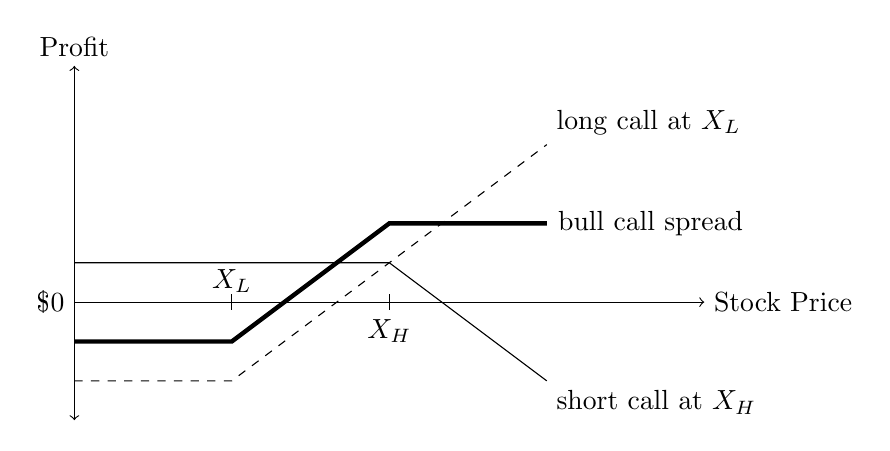
\begin{tikzpicture}
                \draw[<->] (0, -1.5) -- (0, 3) node[above] {Profit};
                \draw[->] (0, 0) node[left] {\$0} -- (8, 0) node[right] {Stock Price};
                \draw[dashed] (0, -1) -- (2, -1) -- (6, 2) node[above right] {long call at $X_L$};
                \draw[ultra thick] (0, -0.5) -- (2, -0.5) -- (4, 1) -- (6, 1) node[right] {bull call spread};
                \draw (0, 0.5) -- (4, 0.5) -- (6, -1) node[below right] {short call at $X_H$};
                \draw (2, 0.1) -- (2, 0) node [above] {$X_L$} -- (2, -0.1);
                \draw (4, 0.1) -- (4, -0.1) node[below] {$X_H$};
            \end{tikzpicture}
        \end{center}
        \begin{align*}
            \text{profit} &= \max(0, S_T - X_L) - \max(0, S_T - X_H) - C_{L, 0} + C_{H, 0}\\
            \text{maximum profit} &= X_H - X_L - C_{L, 0} + C_{H, 0}\\
            \text{maximum loss} &= C_{L, 0} - C_{H, 0}\\
            \text{breakeven price} &= X_L + C_{L, 0} - C_{H, 0}
        \end{align*}
    \end{flushleft}
\end{flashcard}

\begin{flashcard}[\studyArea]{Number of Futures Contracts Needed to Achieve a Target Portfolio Duration}
    \begin{flushleft}
        \begin{align*}
            \text{number of contracts} &= (\text{yield beta}) \left ( \frac{\text{MD}_T - \text{MD}_P}{\text{MD}_F} \right ) \left ( \frac{V_P}{P_f \times \text{multiplier}} \right )\\
            \\
            \text{where:}\\
            V_P &= \text{current value of the portfolio}\\
            P_f &= \text{futures price}\\
            \text{MD}_T &= \text{target modified duration}\\
            \text{MD}_P &= \text{modified duration of the portfolio}\\
            \text{MD}_F &= \text{modified duration of the futures contract}
        \end{align*}
    \end{flushleft}
\end{flashcard}

\begin{flashcard}[\studyArea]{Effects of Gamma on Delta Hedging}
    \begin{flushleft}
        The greater the value of gamma the more risk in the position (i.e., the more variability in the value of the option.)\newline

        The gamma of an at-the-money option is greatest near the expiration. When gamma is large, option values are subject to large changes, the position faces the most risk, and the investor is most likely to use a two-option hedge. In this situation, two options are used to force both delta and gamma to zero.
    \end{flushleft}
\end{flashcard}

\begin{flashcard}[\studyArea]{Interest Rate Caps and Floors}
    \begin{flushleft}
        Interest rate caps and floors are series of interest rate call and put options. Each cap and floor is called a caplet and floorlet.\newline

        Caps and floors are OTC contracts so they're tailored. The terms generally specify
        \begin{itemize}
            \item Reference rate---typically LIBOR.
            \item Cap or floor strike rate.
            \item Length of the agreement.
            \item Reset frequency, whcih determines days in each settlement period, $D_t$.
            \item Notional principal ($\text{NP}$).
        \end{itemize}
    \end{flushleft}
\end{flashcard}

\begin{flashcard}[\studyArea]{Swaps for International Diversification}
    \begin{flushleft}
        Swaps can be used to create international diversification by paying the return on a domestic index and receiving the return on an international index. This creates extra cash flow risk compared to a fixed-receiver swap because of the possibility of both indices declining and having to make two payments.\newline

        Benefits of using these swaps are
        \begin{itemize}
            \item Costs are generally lower than selling domestic and buying international stock.
            \item Can be defined for a temporary period of time for which exposure is desired.
            \item Can be paid in U.S. dollars to avoid foreign currency exposure.
        \end{itemize}
    \end{flushleft}
\end{flashcard}

\cardfrontfoot{Study Session 16}
\renewcommand{\studyArea}{Trading, Monitoring and Rebalancing}

\begin{flashcard}[\studyArea]{Summary of Trading Tactics}
    \begin{tabular}
        {>{\raggedright}p{1.05in}
         >{\raggedright}p{1.05in}
         >{\raggedright}p{1.05in}
         >{\raggedright\arraybackslash}p{1.05in}}
        \toprule

        \textit{Trading Tactic} &
        \textit{Strengths} &
        \textit{Weaknessess} &
        \textit{Usual Trade Motivation}\\ \midrule

        Liquidity-at-any-cost &
        Quick, certain execution &
        High costs and leakage of information &
        Information\\ \addlinespace

        Costs-are-not-important &
        Quick, certain execution at market price &
        Loss of control of trade costs &
        Variety of motivations\\ \addlinespace

        Need-trustworthy-agent &
        Broker uses skill and time to get low price &
        High commission and potential leak of intention &
        Not information\\ \addlinespace

        Advertise-to-draw-liquidity &
        Market-determined price &
        High costs and possible front running &
        Not information\\ \addlinespace

        Low-cost-whatever-the-liquidity &
        Low trading costs &
        Uncertain timing and possible trade into weakness&
        Passive and value\\ \bottomrule
    \end{tabular}
\end{flashcard}

\begin{flashcard}[\studyArea]{Constant Proportion Portfolio Insurance}
    \begin{flushleft}
        Using CPPI, target weight varies with portfolio value and a specified minimum value. The difference is called the cushion. To get target allocation use
        \[
            \text{target investment} = M \times (\text{portfolio value} - \text{floor value} = M \times \text{cushion})
        \]
        where $M$ is the constant proportion for an asset class. To use CPPI, $M$ must be greater than $1$ and it doesn't change once selected.
    \end{flushleft}
\end{flashcard}

\begin{flashcard}[\studyArea]{Performance of Rebalancing Strategies in Different Markets}
    \begin{itemize}
        \item \textbf{Up or down trending market}
            \begin{itemize}
                \item CPPI will outperform. As values increase or decrease, the cushion and resulting allocation increases or decreases, respectively.
                \item Buy-and-hold underperforms CPPI because no purchases or sales are made to capitalize on the changing market values.
                \item Constant mix strategy has the worst performance. Increases in value require selling to bring allocations back to the target. This lowers exposure to future increases in value. The opposite is true for decreases in value.
            \end{itemize}
        \item \textbf{Nontrending, mean-reverting markets}
            \begin{itemize}
                \item CPPI will have the worst performance. A rise in value triggers more allocation, which will then add exposure to an asset that will fall in value. The opposite is true of a fall in value.
                \item Buy-and-hold will perform better than CPPI because no buys or sells are made.
                \item Constant mix has the best performance because increases in value trigger sales at market highs and decreases trigger buys at market lows.
            \end{itemize}
    \end{itemize}
\end{flashcard}

\cardfrontfoot{Study Session 17}
\renewcommand{\studyArea}{Evaluating Portfolio Performance}

\begin{flashcard}[\studyArea]{Strengths and Weaknesses of Micro Attribution and Fundamental Factor Model Attribution}
    \begin{itemize}
        \item \textbf{Micro attribution}
            \begin{itemize}
                \item Strengths
                    \begin{itemize}
                        \item Separates performance between sectors and securities.
                        \item Relatively easy to calculate.
                    \end{itemize}
                \item Weaknesses
                    \begin{itemize}
                        \item Needs an appropriate benchmark with securities and weights at beginning of evaluation period.
                        \item Security selection will affect weighting.
                    \end{itemize}
            \end{itemize}
        \item \textbf{Fundamental factor model attribution}
            \begin{itemize}
                \item Strengths
                    \begin{itemize}
                        \item Identifies factors other than security selection and sector allocation.
                    \end{itemize}
                \item Weaknesses
                    \begin{itemize}
                        \item Factor exposures must be determined at start of evaluation period.
                        \item Can be complex and lead to spurious correlation.
                    \end{itemize}
            \end{itemize}
    \end{itemize}
\end{flashcard}

\begin{flashcard}[\studyArea]{Diagram of Risk-Adjusted Measures}
    \begin{flushleft}
        \begin{center}
            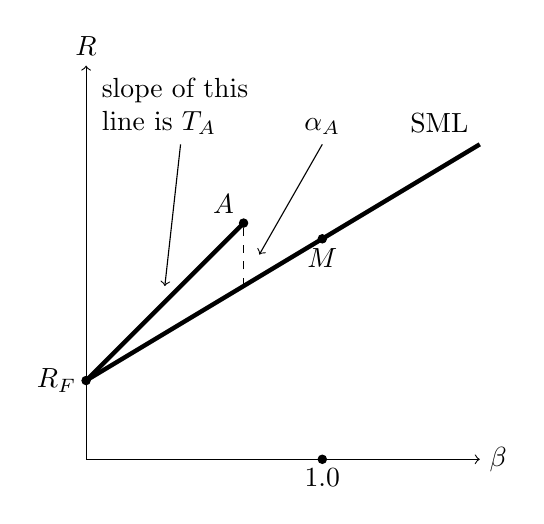
\begin{tikzpicture}
                \draw[->] (0, 0) -- (0, 5) node[above] {$R$};
                \draw[->] (0, 0) -- (5, 0) node[right] {$\beta$};
                \draw[ultra thick] (0, 1) -- (5, 4) node[above left] {SML};
                \draw[ultra thick] (0, 1) -- (2, 3);
                \draw[dashed] (2, 2.2) -- (2, 3);
                \draw[->] (3, 4) node[above] {$\alpha_A$} -- (2.2, 2.6);
                \draw[->] (1.2, 4) node[above, text width=2cm] {slope of this line is $T_A$} -- (1, 2.2);
                \draw[fill] (0, 1) circle[radius=1.5pt] node[left] {$R_F$};
                \draw[fill] (2, 3) circle[radius=1.5pt] node[above left] {$A$};
                \draw[fill] (3, 2.8) circle[radius=1.5pt] node[below] {$M$};
                \draw[fill] (3, 0) circle[radius=1.5pt] node[below] {1.0};
            \end{tikzpicture}
            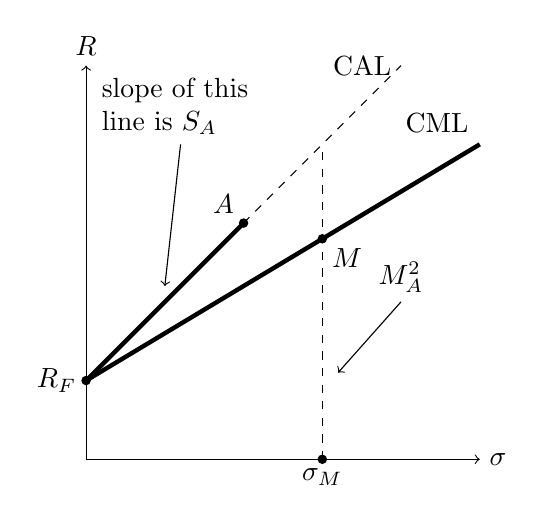
\begin{tikzpicture}
                \draw[->] (0, 0) -- (0, 5) node[above] {$R$};
                \draw[->] (0, 0) -- (5, 0) node[right] {$\sigma$};
                \draw[ultra thick] (0, 1) -- (5, 4) node[above left] {CML};
                \draw[ultra thick] (0, 1) -- (2, 3);
                \draw[dashed] (2, 3) -- (4, 5) node[left] {CAL};
                \draw[dashed] (3, 0) -- (3, 4);
                \draw[->] (4, 2) node[above] {$M^2_A$} -- (3.2, 1.1);
                \draw[->] (1.2, 4) node[above, text width=2cm] {slope of this line is $S_A$} -- (1, 2.2);
                \draw[fill] (0, 1) circle[radius=1.5pt] node[left] {$R_F$};
                \draw[fill] (2, 3) circle[radius=1.5pt] node[above left] {$A$};
                \draw[fill] (3, 2.8) circle[radius=1.5pt] node[below right] {$M$};
                \draw[fill] (3, 0) circle[radius=1.5pt] node[below] {$\sigma_M$};
            \end{tikzpicture}
        \end{center}
    \end{flushleft}
\end{flashcard}
\end{document}
